
\section{Plugin}
In order to improve the deployment and usage of the refactoring tool a plugin
for DrRacket was created.
DrRacket has several advantages and the plugin support is another one, because
it allows a simple integration with DrRacket itself a simple managing interface.
Another advantage is the incorporation with git. A plugin can be a link for a git
repository and because of that it becomes simple to keep the refactoring tool up to date.

However, the main reason to create a plugin is to become independent from DrRacket
evolution. With a plugin that is possible and it is manageable.
\section{FrameWork}
Python: [framework]
One of the goals of this thesis is to create refactoring for dynamic languages in general,
in other words, to create a Framework for refactoring tools.
//by using the same structure (program, framework, choose one better)
After creating several refactoring operations for Racket Python was chosen next.
POC (prove of concept)
It was created a prove of concept in Python consistent in several refactoring operations, such as:
[TODO] say which refactoring operations were implemented.
Python was chosen because there is already an implementation of Python for the
 DrRacket environment in which the refactoring tool for Racket was first developed.

%[TODO say what parts of the code were reused]

 %[TODO Explain META-LANGUAGE]
 The implementation for DrRacket is what does the trick, because by implementing
 the language with Racket syntax we use it as a meta-language which then
 can represent several different languages. Being the meta-language a language that are
 composed only by syntax elements is a huge advantage to compute effortless new
 refactoring operations for new languages when compared with the necessary effort to create
 the refactoring operations directly for that language.

Ideally we should only have refactoring operations for the meta-language which represents
all languages. And then specialized pretty printers to output the changes in the
desireble language.
However, since we instead of having a general representation that can represent all the languages
supported we have the languages represented in Racket's syntax objects we can not do that.

We indeed have a meta-language that abstracts all the supported languages and
we have trully language independent refactoring operations. However, it is only
for a small set of refactoring opeartions, the more simple ones. We did it like
this because we would lose some of the possible refactoring operations or we would
have to have a lot of concerns. And since we have a restrict amount of time, having
a meta-language that have language-independent refactoring operations combined
with the "semi-meta-languages" that have similar refactoring operations but
language dependent and therefore more specialized.

With this we do not have a language-independent framework. However we have a framework
for refactoring operations, even tough that is more aimed at dynamic and functional languages.
Framework architecture.
\begin{figure}[h]
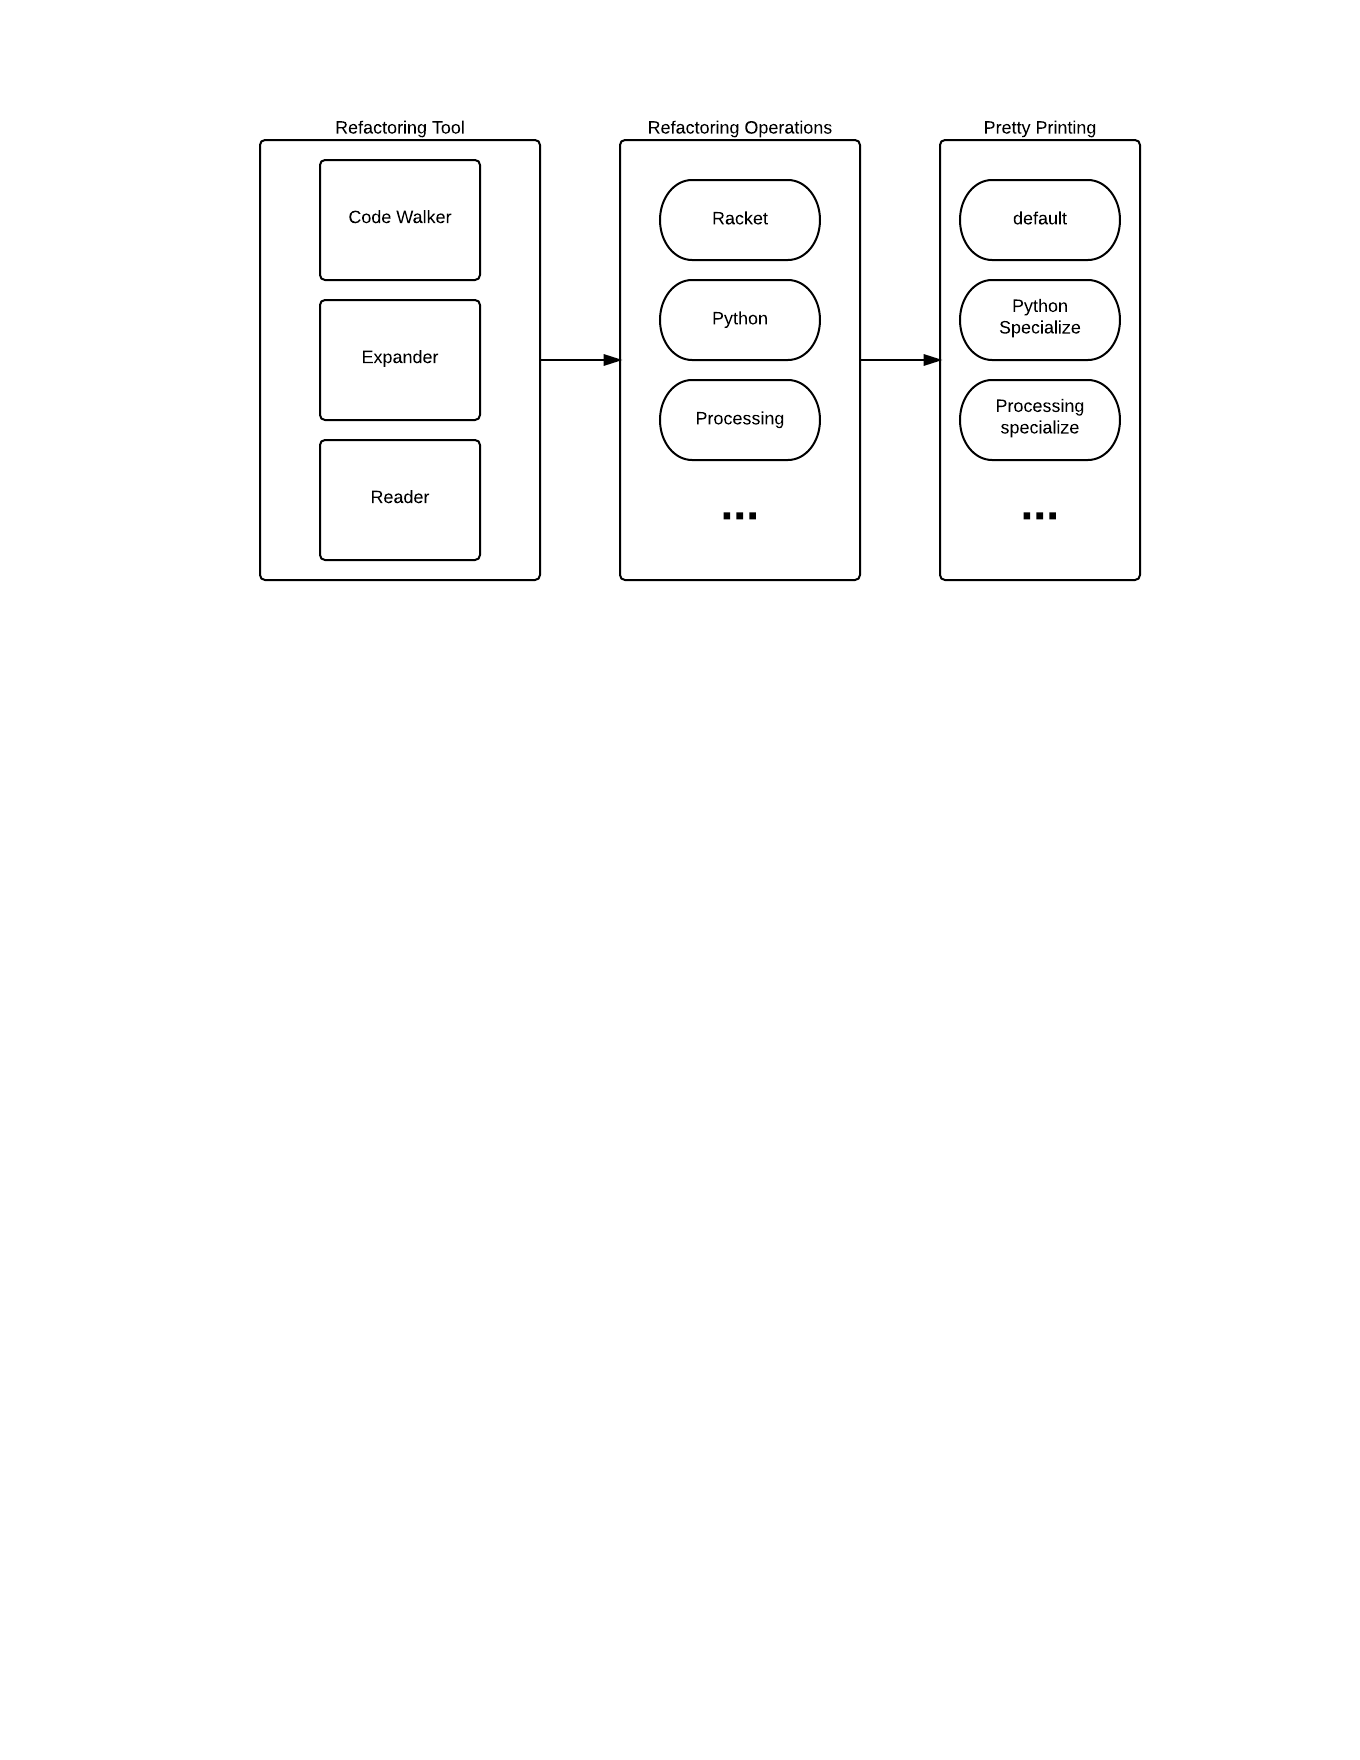
\includegraphics[width=8cm]{../framework-arch.png}
\end{figure}

\subsection{Statement based languages}
This Framework was build with a base of expression based languages. The flow of
the program is needed to decide whether or not a refactoring can be correctly done
or even to decide where and how many returns a function needs. However this could
be minimized with a PDG (program depedence graph) that has the control flow information
needed to compute correct refactorings.

\section{Features}
how easy it is to add new refactoring operations and languages
The framework it is simply to use, it is only necessary to have a specification file
of each refactoring operation.
That file must have a function that receives two arguments,
one is the AST of the program and the other is the def-use-relation.
This information makes it possible to have several refactoring operations that help
the programmer.
what was "reused"
everything except the refactoring operations itself.
the advantages of that
This Framework makes it easier to implement refactoring operations for dynamic languages,
with only the catch that they have to be implemented for DrRacket. Helping minimizing
the problem of the difficulty and lacking of refactoring operations for dynamic languages.
(for at least every language implemented for DrRacket)
\section{Tool Maintenance} %Framework maintenance!
%Developer Point of view
%%%% Nor for the paper tough %%%%
%%automatic might help save work when the user nows what exactly the tool will do.

%This feature combined with the automatic suggesting is a huge help to do the
%evaluation of this refactoring tool and to use in battery tests.


%FIXME change to the FRAMEWORK
A refactoring tool is a quite complex piece of software and therefore requires maintenance.
Automatic testing is used in general by developers to ensure that the software
is bug free for those test cases.
By having a way to automatically perform all the refactoring operations found,
the developer of a refactoring tool can test and ensure if the changes made did not introduce
bugs in other refactoring operations of the refactoring tool.
One way to automatic test the refactoring operations is to apply every refactoring
operations possible to a piece of code. By having this possibility it is simpler
to the developer to create specific test cases that simplify tool maintenance.
In order to do this it is necessary to correctly identify all the possible refactoring
operations in one piece of code. Such operation is already implemented in the refactoring
tool, the automatic suggesting.
Therefore the remaining part of the algorithm is to apply all of those operations.
The trick part is  that every refactoring operation changes the AST, so after
applying one refactoring operation it is necessary to recompute the program AST.
By changing the AST the possible refactoring operations applicable also might change,
so it is necessary to recompute the AST.

%First the automated refactoring displays all the possible refactoring found thus making it easier
%to detect the refactoring operations in projects.
%It makes it easier to evaluate the need to do the refactoring and to evaluate
%if the refactoring tool (frameowork) is working correctly.
%Second the automatic refactoring makes it easier to test if the refactoring operations are correct (**** for a limited test cases ****)
%This is possible by running the test cases of the program before any refactoring.
%Then using automatic refactoring in the program that applies all the refactoring that the tool finds.
%And finally by running again the test cases of the program.
%After testing it with several (or huge) programs if every test passes (or the exact same tests, because refactoring operations should not fix bugs)
%we can consider that the refactoring operations are correct.
\section{Analysis}
\subsection{Famix}

\section{Conclusion}
\section{Future Work}
Add a PDG to the framework.
